\chapter{\NAME in detail}
\label{s:aquagpusph}
%
\section{General}
\label{ss:aquagpusph:general}
%
\NAME functionality can be deeply analyzed using Doxygen documentation. In section \ref{s:install}
you can find how to build Doxygen developers documentation during \NAME compile process. When \NAME
have been already built you can open Doxygen documentation web page with your internet browser,
loading doc/Doxygen/html/index.html web page file.\rc
%
The objective of this chapter is provide some key notes about how \NAME works in order to allow users
understand well what can do or not with this software.\rc
%
In figure \ref{fig:aquagpusph:generalDiagram} you can see the general flux diagram. \NAME is based on a
host-server structure. Host is designed to prepare the case, and to receive and process results, since
server is designed to receive data from server, and compute as many time steps as possible until no new
output is needed.\rc
%
This structure does not only simplify the process and allows more comprehensive code, also is designed
for tolerate several calculation servers working simultaneously on future releases, trying to preserve
the actual simplicity.
%
\begin{figure}[ht!]
  \centering
  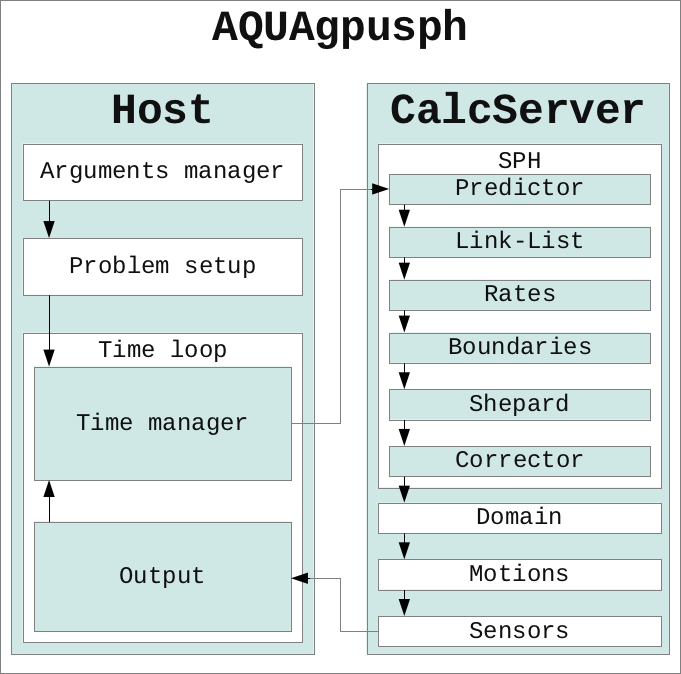
\includegraphics[width=0.7\textwidth]{GeneralDiagram}
  \caption{General \NAME flux diagram}
  \label{fig:aquagpusph:generalDiagram}
\end{figure}
%
\section{Arguments manager}
\label{ss:aquagpusph:argmanager}
%
Arguments manager is the piece of code that analyse input command line options/arguments. You can get a
list of valid options and arguments executing:
%
\begin{verbatim}
AQUAgpusph --help
\end{verbatim}
%
Valid options are:
%
\begin{itemize}
	\item \textbf{-i, -\--input=INPUT}: Set the definition XML file of the simulation.
	\item \textbf{-o, -\--output-prefix=PREFIX}: Set a prefix for output files.
	\item \textbf{-n, -\--no-reassembly}: Visualization output files will not reassembled.
	\item \textbf{-v, -\--version}: Show \NAME version and stop the execution.
	\item \textbf{-h, -\--help}: Show \NAME helps page and stop the execution.
\end{itemize}
%
Options can be freely used simultaneously until incompatibilities are not notified here, or at the help
page. Some combinations of command line options can result on undesired behaviour, like for instance
mixing -\--version with -\--help will discard one of them.\rc
%
In almost cases -\--no-reassembly is a good option, due to reassembly output files can be a really
hard-disk \& CPU consuming process.
%
\section{Problem setup}
\label{ss:aquagpusph:problemsetup}
%
The problem setup stage basically consist on loads all settings established as explained on chapter
\ref{s:caseSetup}, and load the particles/vertexes data from described files on chapter \ref{ss:partsFile}.\rc
%
Problem setup will report work done, and the eventually incidences, on the initialization screen output.
The screen output during initialization and close stages of \NAME execution will be preserved if NCurses
support has been activated, but if NCurses support is not active you can lost the initialization process
reported messages due to the large amount of these printed during the simulation. In this case you
can redirect the screen output to a file typing:
%
\begin{alltt}
AQUAgpusph \emph{COMMANDLINE_OPTIONS} > screen.out
\end{alltt}
%
You can also detach the execution from terminal, for instance using:
%
\begin{alltt}
nohup AQUAgpusph \emph{COMMANDLINE_OPTIONS} > screen.out &
\end{alltt}
%
Allowing you to run \NAME remotely, but in this case you will lost the possibility of stop simulation using `c'
key\footnote{Advanced Linux users can get the process PID and then reinject keys to program}, that as described
on chapter \ref{ss:running:launching} allows you to right stop the simulation closing files.\rc
%
In both cases you will preserve a file called ``screen.out'' that saves the messages reported during
initialization and close stages, and along the simulation as well.
%
\section{Leap-Frog integration scheme}
\label{ss:aquagpusph:leapfrog}
%
Weakly compressible SPH method is able to return the instantaneous acceleration and density rate for each
particle in a Lagrangian point of view, so 3 variables must be integrated along the time, velocity, position
and density of each particle. \NAME time integration is based on a Leap-Frog predictor-corrector scheme:
%
\begin{enumerate}
	\item Predictor:
	\[
	\dot x_{t+dt}^{\mathrm{pred}} = 
	\dot x_{t} + 
	dt \left(
		\ddot x_{t} + g
	\right)
	\]
	\[
	x_{t+dt}^{\mathrm{pred}} = 
	x_{t} + 
	dt \dot x_{t} + 
	\frac{dt^2}{2} \left(
		\ddot x_{t} + g
	\right)
	\]
	\[
	\rho_{t+dt}^{\mathrm{pred}} = 
	\rho_{t} + 
	dt \dot\rho_{t}
	\]
	\item SPH interactions:
	\[
	\ddot x_{t+dt} \leftarrow \mbox{SPH}
	\]
	\[
	\dot\rho_{t+dt} \leftarrow \mbox{SPH}
	\]
	\item Corrector:
	\[
	\dot x_{t+dt} = 
	\dot x_{t+dt}^{\mathrm{pred}} + 
	\frac{dt}{2} \left(
		\ddot x_{t+dt} - \ddot x_{t}
	\right)
	\]
	\[
	x_{t+dt} = x_{t+dt}^{\mathrm{pred}}
	\]
	\[
	\rho_{t+dt} = 
	\rho_{t+dt}^{\mathrm{pred}} + 
	\frac{dt}{2} \left(
		\dot\rho_{t+dt} - \dot\rho_{t}
	\right)
	\]
\end{enumerate}
%
\section{Link-List}
\label{ss:aquagpusph:linklist}
%
SPH codes commonly uses a PIC (Particle In Cell) based algorithm to easily locate particle's neighbours, called
Link-List. The main difference with typical PIC algorithm is that on SPH a chain is built from the cells data,
linking each particle with the next one on the same cell, allowing that cell only saves the index of the
first particle of the chain.\rc
%
In figure \ref{fig:aquagpusph:LinkList} a simplified scheme of Link-List stored data is shown. Particles are
located in cells that have a length of the maximum interaction distance, then each cell allocates a particle
index called ``head of chain'' (\textit{ihoc}). Each particle stores the next one of the cell chain (\textit{ll})
until last particle is reached, where some invalid index is set  (-1 for instance).\rc
%
In GPU oriented code this behaviour can be conveniently modified looking for sorted memory address reading, that
is really more efficient, sorting particles by cell index. The problem is that traditional method implies storing
Link-List chain, and more over, implies a chaotic memory access at particles interaction stage, with a heavy
performance penalty. So, as many other GPU based SPH codes, \NAME sorts the particles, transforming the Link-List
array ll[\textit{i}] in \textit{i}+1 variables, so is not anymore needed to store it therefore.\rc
%
\begin{figure}[h!]
  \centering
  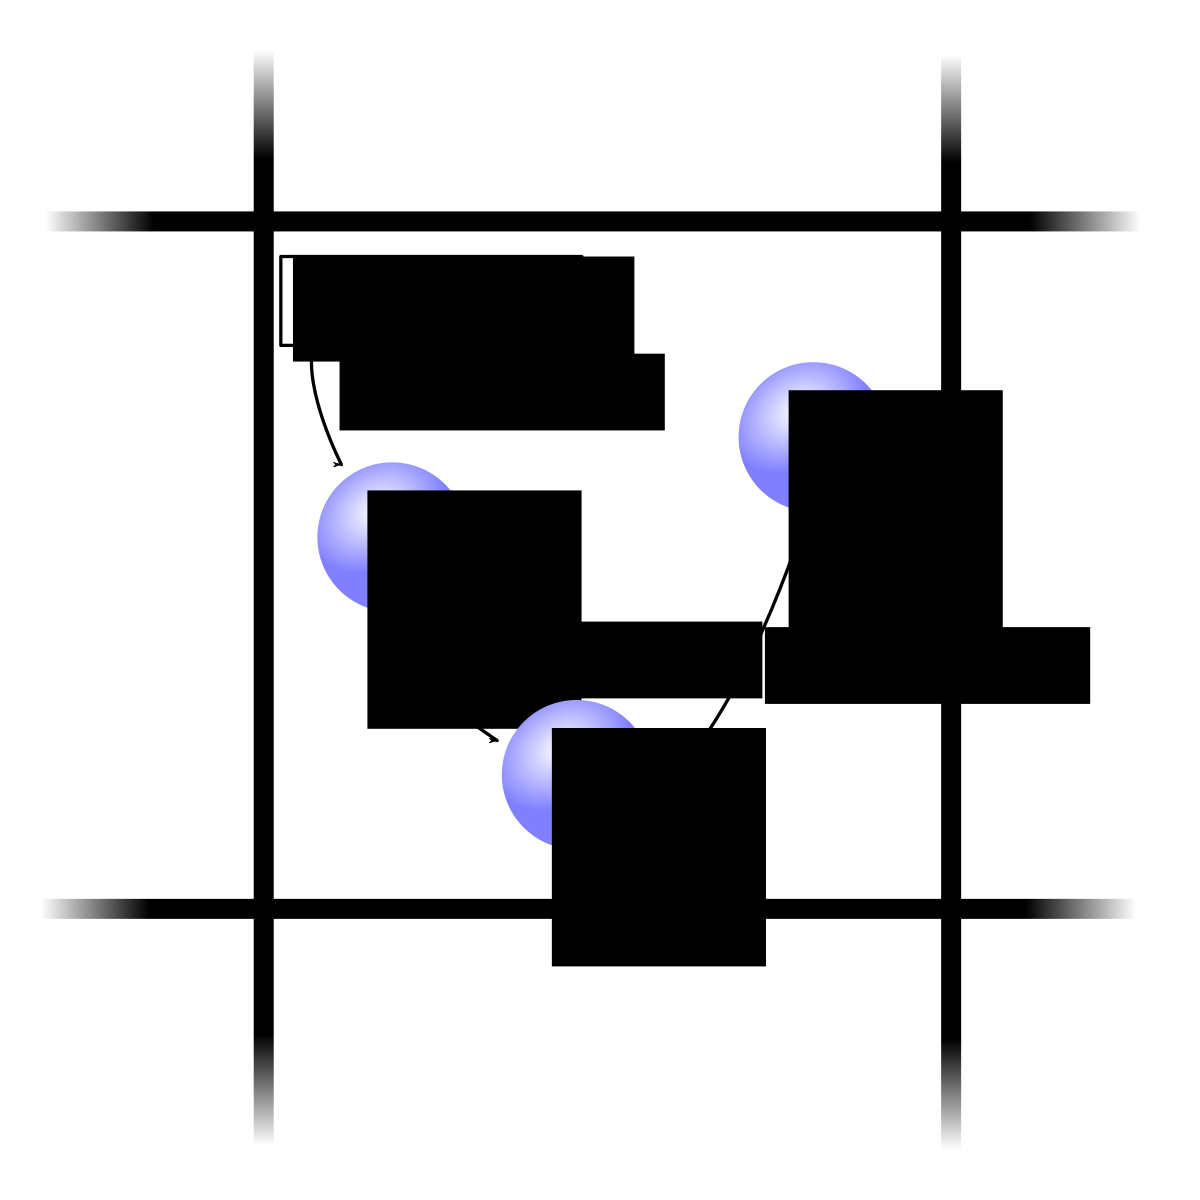
\includegraphics[width=0.7\textwidth]{LinkList}
  \caption{Conventional Link-List scheme}
  \label{fig:aquagpusph:LinkList}
\end{figure}
%
\section{Particles interactions}
\label{ss:aquagpusph:rates}
%
Particles interactions is the core of every SPH method, and is the most complex stage too, being the most
time consuming one. \NAME can perform several particles interaction stages by time step depending on simulation
settings, for instance, if `DeLeffe' boundary condition is set at least 3 interactions stages will be performed,
the usual one, the boundary integrals, and `ElasticBounce' non wall trespassing condition, but since only the usual one
needs to compute all possible particles interactions, the others may take less time.\rc
%
As explained in section \ref{ss:aquagpusph:linklist}, the particles interactions computation performance is
heavily dependant on Link-List stage and \NAME performs a particles sorting based on cell as many other GPU
oriented SPH codes, but two main differences must be remarked:
%
\subsection{Unsorted output arguments}
%
In section \ref{ss:aquagpusph:leapfrog} time integration scheme is described, and we can find that after predictor
stage, variables $\dot x_{t}$, $\mathbf{x}_{t}$, and $\rho_{t}$ are not needed anymore until new time step,
so \NAME can use these arrays in order to store sorted data for SPH interactions stage, decreasing memory
requirements, but the same process can not be applied to output data $\ddot x_{t}$ and $\dot\rho_{t}$,
because is needed on corrector stage, so there are 2 ways to solve it:
%
\begin{enumerate}
	\item Create new arrays for the sorted output data, working all time in sorted space.
	\item Work on sorted space, but write at unsorted space.
\end{enumerate}
%
\NAME use the second way, that have some significant advantages:
%
\begin{enumerate}
	\item Less memory requirements that the first way.
	\item Since \NAME is using non needed arrays to store the sorted input data, the unsorted data is preserved.
	\item Since the output data is written on unsorted space directly, after SPH interactions stage all the
	unsorted data is available to continue working, including to print output files (Note that the unsorted space
	is the original one).
	\item No unsort operation is required.
\end{enumerate}
%
Of course, write into the unsorted space at the interactions stage can be more expensive, but since the writing
operations are really less frequent than the reading ones, performance decrease can be assumed.
%
\subsection{Coalescence read}
%
Newest hardware not suffers really heavy penalties when a lot of threads try to read from the same memory address,
nevertheless \NAME incorporates an algorithm in order to reduce as much as possible the number of readers over
unique address. In figure \ref{fig:aquagpusph:CoalescenceRead} a scheme about the interactions process is shown.
Interactions stage is divided in 3 substages:
%
\begin{enumerate}
	\item Interacts with next particles of the home cell\footnote{Home cell is the cell where the computing
	particle is located} chain.
	\item Interacts with the particles on the neighbour cells.
	\item Interacts with previous particles of the home cell chain.
\end{enumerate}
%
As you can see in figure \ref{fig:aquagpusph:CoalescenceRead} the particles does not reads from the same memory
address in any interactions. In practice, due to the particles interactions can take different times, due to the
neighbour cells particles can try to read from same memory address, several simultaneous reads can happens, but
in much less number.
%
\begin{figure}[ht!]
  \centering
  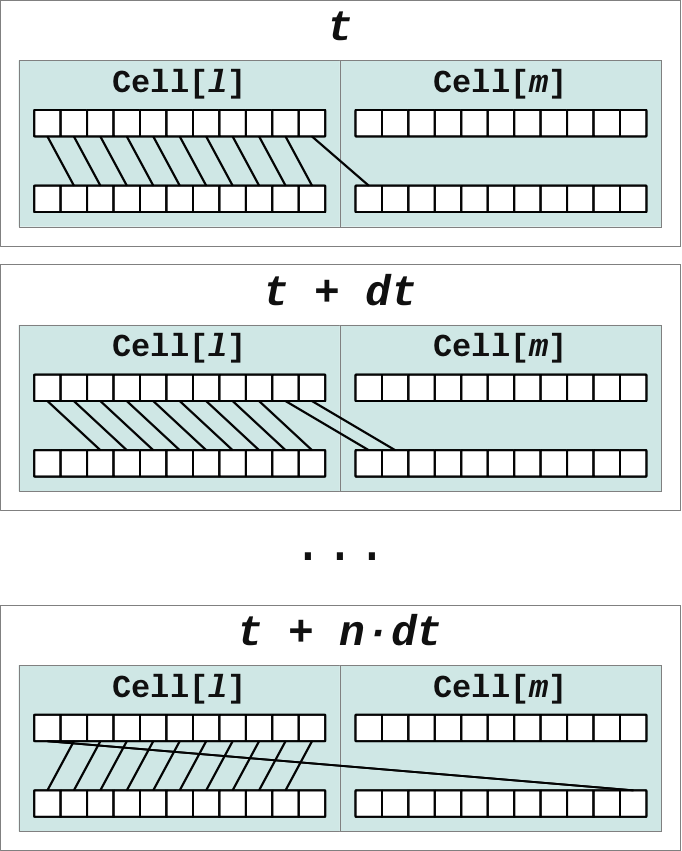
\includegraphics[width=0.7\textwidth]{CoalescenceRead}
  \caption{Coalescence reading flow}
  \label{fig:aquagpusph:CoalescenceRead}
\end{figure}
%
\section{Boundary conditions}
\label{ss:aquagpusph:boundaries}
%
\subsection{General}
%
\NAME provides most commonly used boundary conditions in order to allow users to can choose the one than better fit
to their problem. The generally suggested method is Boundary integrals (formerly `DeLeffe') that is flexible and
powerful, but have the disadvantage that requires `Shepard' correction for consistency.\rc
%
Along this chapter all boundary conditions will be described, and advantages discussed. Also the mixing possibilities
will be introduced.
%
\subsection{Elastic bounce}
\label{sss:aquagpusph:boundaries:elasticbounce}
%
This is the simplest way to impose the boundary conditions, based on particle elastic bound within the wall, where
a elastic factor is applied in order to set plasticity.\\
%
In figure \ref{fig:aquagpusph:BounceScheme} a scheme of the elastic bound effect is shown. In \NAME walls are
defined by a set of vertexes (black balls), that have a normal\footnote{Ensure yourself that the provided normals
are normalized, \NAME will accept it as set by user} and area associated (area is stored on mass array).
In order to \NAME identify particles as vertexes, $imove$ flag must be set lower than 0.\\
%
Elastic bounce is applied when a particle will moved nearer to a vertex than `BoundDist' parameter introduced on
chapter \ref{sss:XML:SPH}, then the normal component of velocity is modified in order to get an elastic bound
multiplied by elastic factor `BoundElasticFactor'. If the elastic factor is 1, a fully elastic bound will
performed, however if elastic factor is 0, particle will stopped (normal component of the velocity will affected
only), so with values between 0 and 1 a semi-elastic bound will performed. You can set elastic factors out of
[0,1] bounds if you know what are you doing.\\
%
Main advantage of this boundary is the simplicity that reverts on a good performance, but using the Elastic bounce
boundary condition alone will return poor physics results, The Elastic bounce boundary condition is then aimed to
work with other boundary conditions, serving a second barrier for particles that can try to trespass the walls.
%
\begin{figure}[h!]
  \centering
  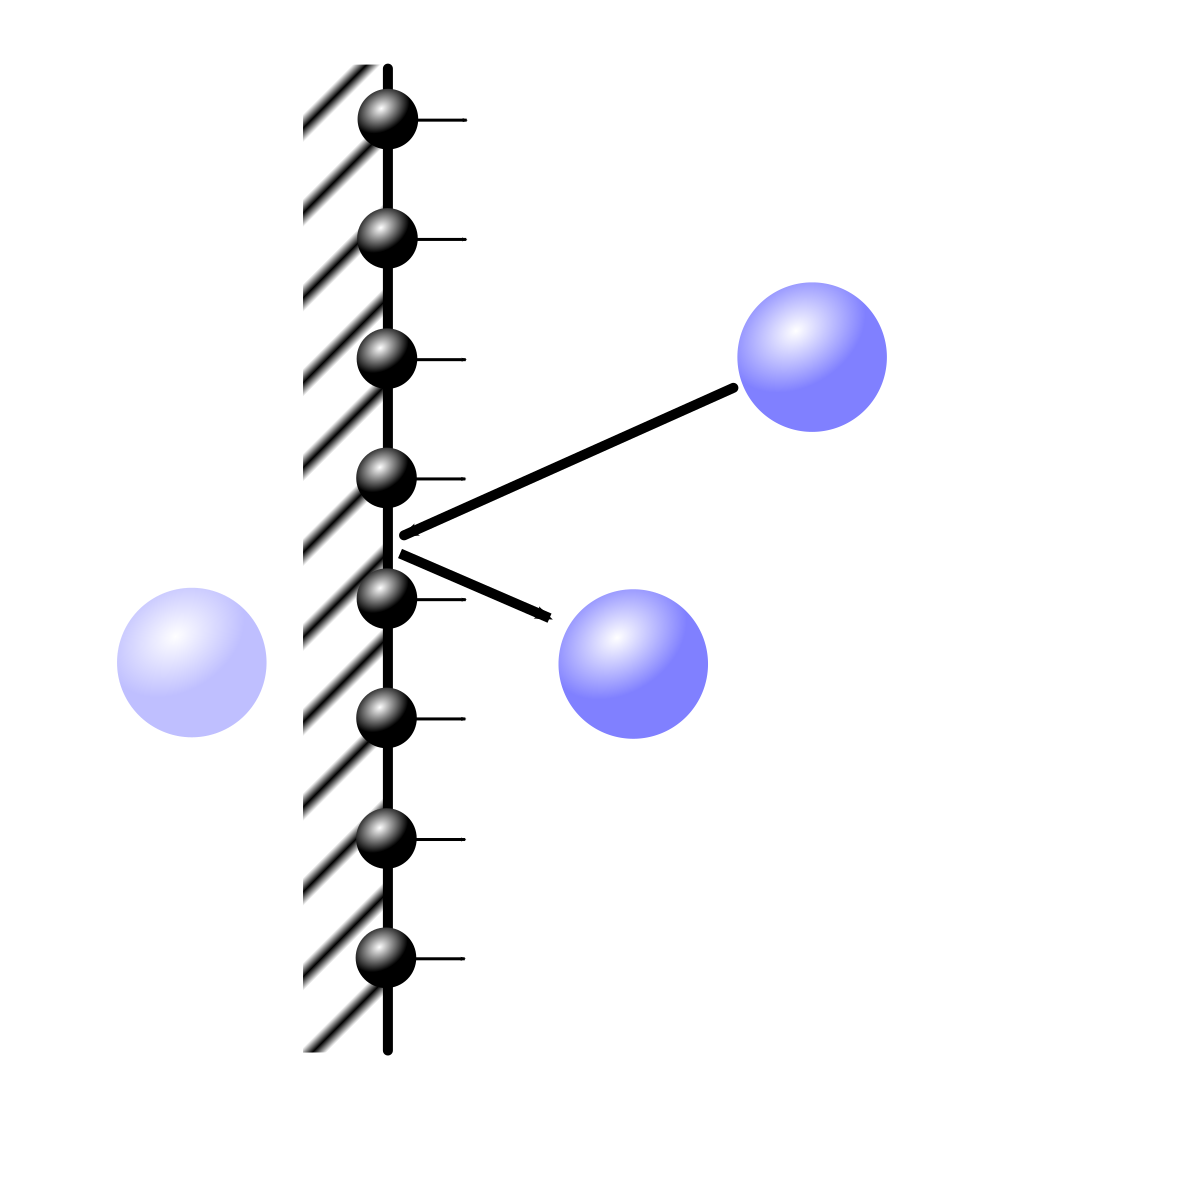
\includegraphics[width=0.25\textwidth]{ElasticBounce}
  \caption{Elastic bounce boundary scheme}
  \label{fig:aquagpusph:BounceScheme}
\end{figure}
%
\subsection{Fix particles}
\label{sss:aquagpusph:boundaries:fixparticles}
%
`Fix particles', also called `dummy particles' sometimes, is a extension of the fluid domain along walls with a little
bit especial fluid particles linked to them.\\
%
In figure \ref{fig:aquagpusph:FixParticlesScheme} an scheme of the fixed particles distribution is shown. Must be
noticed that first row of fixed particles is placed \textit{dr}/2 inner on wall, and the several rows are placed
every \textit{dr}. The fixed particles are similar to the fluid ones, but a normal must be provided and
\textit{imove} flag must be lower than 0.\\
%
The fixed particles will use continuity equation like the fluid particles, but not momentum equation, because
fixed particles velocity is linked to the wall motion. Related to this, if no motions are set, the initial fixed
particles velocity will be preserved along the simulation\footnote{you can modify this behaviour with custom
predictor and corrector kernels}.\\
%
SPH equations when `Fix particles' boundary condition is used are therefore
%
\[
\left. \left\langle \frac{\gradient p}{\rho} \right\rangle_a \right\vert_{a \in \mathrm{Fluid}} = \frac{1}{\gamma_a}
	\sum\limits_{b \in \mathrm{Fluid}\;\cup\;\mathrm{Boundary}} 
		\left( \frac{p_a}{\rho_a^2} + \frac{p_b}{\rho_b^2} \right)
	\gradient W_{ab} m_b
\]
%
\[
\left. \left\langle \rho \; \divergence(v) \right\rangle_a \right\vert_{a \in \mathrm{Fluid}\;\cup\;\mathrm{Boundary}} =
	- \frac{1}{\gamma_a}
	\sum\limits_{b \in \mathrm{Fluid}\;\cup\;\mathrm{Boundary}} 
		\left( v_a - v_b \right)
	\gradient W_{ab} m_b
\]
%
\[
v_{a \in \mathrm{Boundary}} = \mathrm{f}\left(x_\mathrm{walls} \left( t \right) \right)
\]
%
Where $\gamma_a$ can be forced to be 1 ever setting Shepard correction to ``None'' as decribed on the chapter
\ref{sss:XML:SPH}, that have the advantage of getting a fully conservative notation.\\
%
`Fix particles' uses internally `ElasticBounce boundary' condition described on section
\ref{sss:aquagpusph:boundaries:elasticbounce}. It's strongly recommended let `Fix particles' work with
`ElasticBounce boundary' in order to warranty that the particles can trespass the walls, but if you want to
disable this feature simply set `BoundDist' parameter to 0, \textbf{never pass null normals to the fixed
particles}.\\
%
`Fix particles' is chronologically the first boundary condition implemented on SPH, has the main advantage that is
easy to implement since the fixed particles have a really similar treatment to the usual fluid particles, but
have the main disadvantage of the particles velocity set using only walls motion as a `U0M', that gives an
inconsistent Laplacian operator. Also requires increase the number of particles significantly, more as the number of neighbours grows.
%
\begin{figure}[ht!]
  \centering
  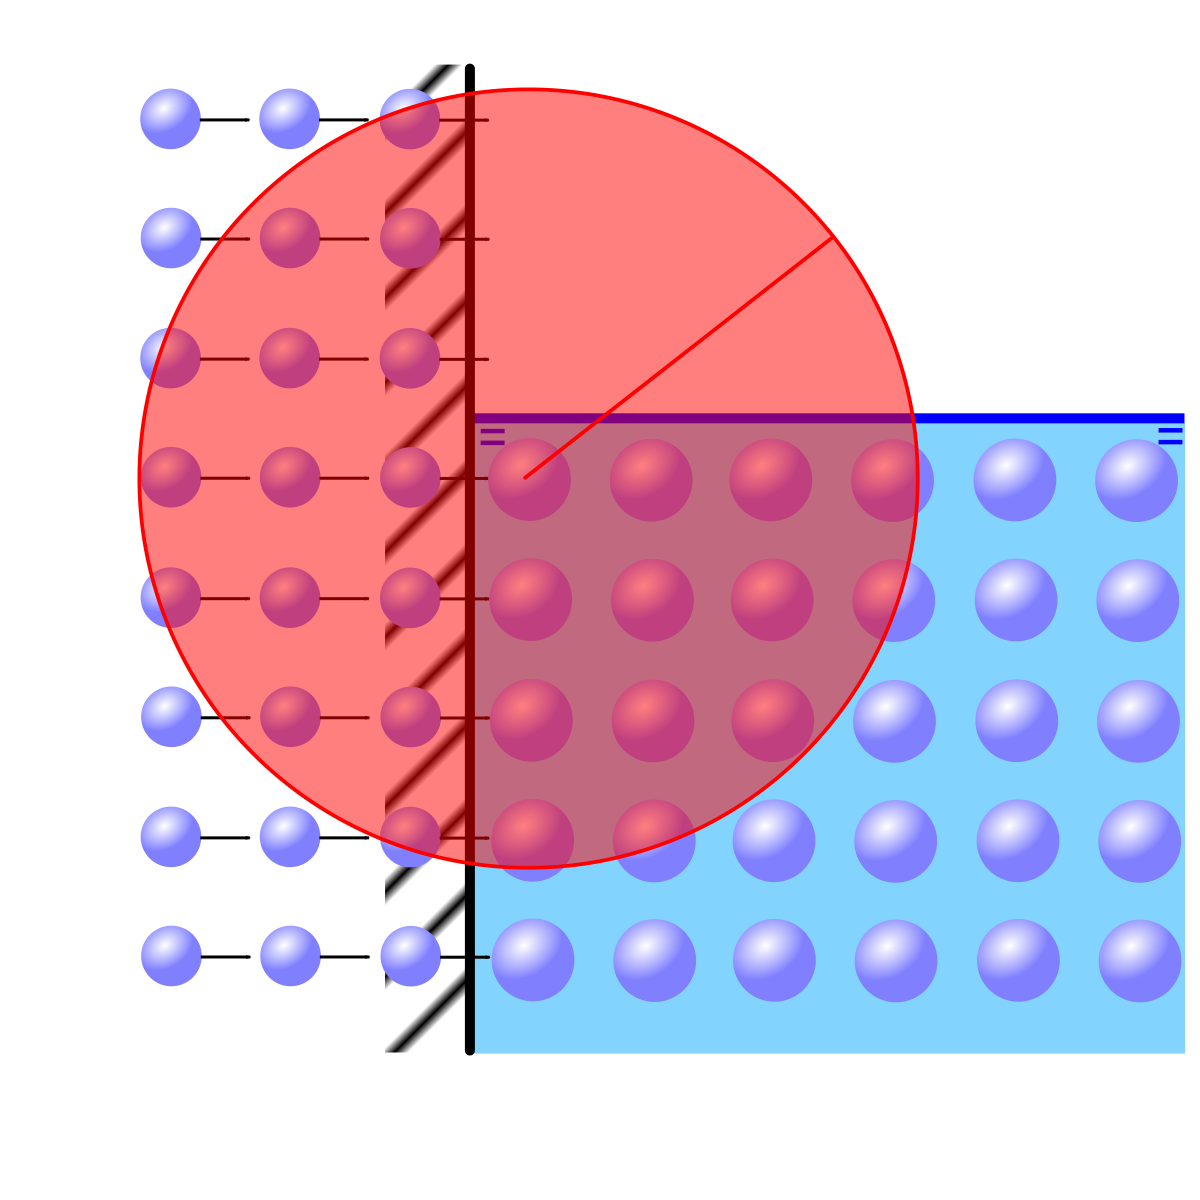
\includegraphics[width=0.4\textwidth]{FixedParticles}
  \caption{Fix particles scheme}
  \label{fig:aquagpusph:FixParticlesScheme}
\end{figure}
%
\subsection{Boundary integrals, formerly `DeLeffe'}
\label{sss:aquagpusph:boundaries:DeLeffe}
%
Boundary integrals is the newest method to compute boundary conditions, and the implementation method is similar
to `ElasticBounce boundary' described at section \ref{sss:aquagpusph:boundaries:elasticbounce}.\\
%
In figure \ref{fig:aquagpusph:DeLeffeScheme} a boundary integrals scheme is shown. In original DeLeffe's boundaries
integral development, oriented to 2D applications, an analytic solution of the integral, with a discretized
version of fields, is purposed for full integration line (green highlighted on the image). In \NAME each vertex
is associated to a wall area, then not only the field is discretized but also the integral as well, with a little
bit worst result, but allowing to use this method in 3D simulations too.\\
%
In order to can converge the discretized boundary integral to the analytical one, you can set more vertexes with
smaller areas, but be mindful that the values in vertexes along the walls are interpolated from the fluid particles,
so really high resolution in walls, compared to fluid resolution, don't make any sense due to bad interpolated
fields.\\
%
Boundary integrals have advantages in terms of consistency, with consistency of order $\mathcal{O}(h)$ for all the
operators, including the Laplacian. At the other hand this boundary condition requires Shepard correction, that
can be a little bit unstable, and breaks the fully conservative SPH notation. The equations are therefore
%
\[
\left. \left\langle \frac{\gradient p}{\rho} \right\rangle_a \right\vert_{a \in \mathrm{Fluid}} =
	\frac{1}{\gamma_a} \left(
		\sum\limits_{b \in \mathrm{Fluid}} 
			\left( \frac{p_a}{\rho_a^2} + \frac{p_b}{\rho_b^2} \right)
		\gradient W_{ab} m_b
		- \sum\limits_{b \in \mathrm{Boundary}}
			\rho_b \left( \frac{p_a}{\rho_a^2} + \frac{p_b}{\rho_b^2} \right)
		n_b S_b
	\right)
\]
\[
\left. \left\langle \rho \; \divergence(v) \right\rangle_a \right\vert_{a \in \mathrm{Fluid}} =
	- \frac{1}{\gamma_a} \left(
		\sum\limits_{b \in \mathrm{Fluid}} 
			\left( v_a - v_b \right)
		\gradient W_{ab} m_b
		- \sum\limits_{b \in \mathrm{Boundary}}
			\rho_b \left( v_a - v_b \right)
		n_b S_b
	\right)
\]
\[
p_{a \in \mathrm{Boundary}} = \sum\limits_{b \in \mathrm{Fluid}}
	\left( \frac{p_b}{\rho_b} + g \cdot r_{ab}\right )
	W_{ab} m_b
\]
\[
v_{a \in \mathrm{Boundary}} = \mathrm{f}\left(x_\mathrm{walls} \left( t \right) \right)
\]
%
Since the integration domain is truncated (this method is not based on a fluid extension), Shepard correction usage
is mandatory. In \NAME Shepard correction over the pressure term will be applied by default, but not over the
continuity equation, because compressibility is small in all cases, and Shepard correction can unstabilize this
equation. Nevertheless you can activate the Shepard normalization as described in the chapter \ref{sss:XML:SPH}.\\
%
Must be noticed that the vertexes must be placed on the center of their representative area, taking special care on
the limits of walls. In figure \ref{fig:aquagpusph:DeLeffeCorner} the distribution of vertexes, that is separated 
\textit{dr}/2 (half of distance between particles \textit{dr}), in a corner is shown. Since the area (line length
because is a 2D example) associated to each vertex is \textit{dr}/2, the distance of first vertex to corner is
\textit{dr}/4.\\
%
`DeLeffe' uses internally `ElasticBounce boundary' condition described on section
\ref{sss:aquagpusph:boundaries:elasticbounce}. It's strongly recommended let `DeLeffe' work with
`ElasticBounce boundary' in order to warranty that the particles can trespass the walls, but if you want to
disable this feature simply set `BoundDist' parameter to 0, \textbf{never pass null normals to the vertexes}.
%
\begin{figure}[h!]
  \centering
  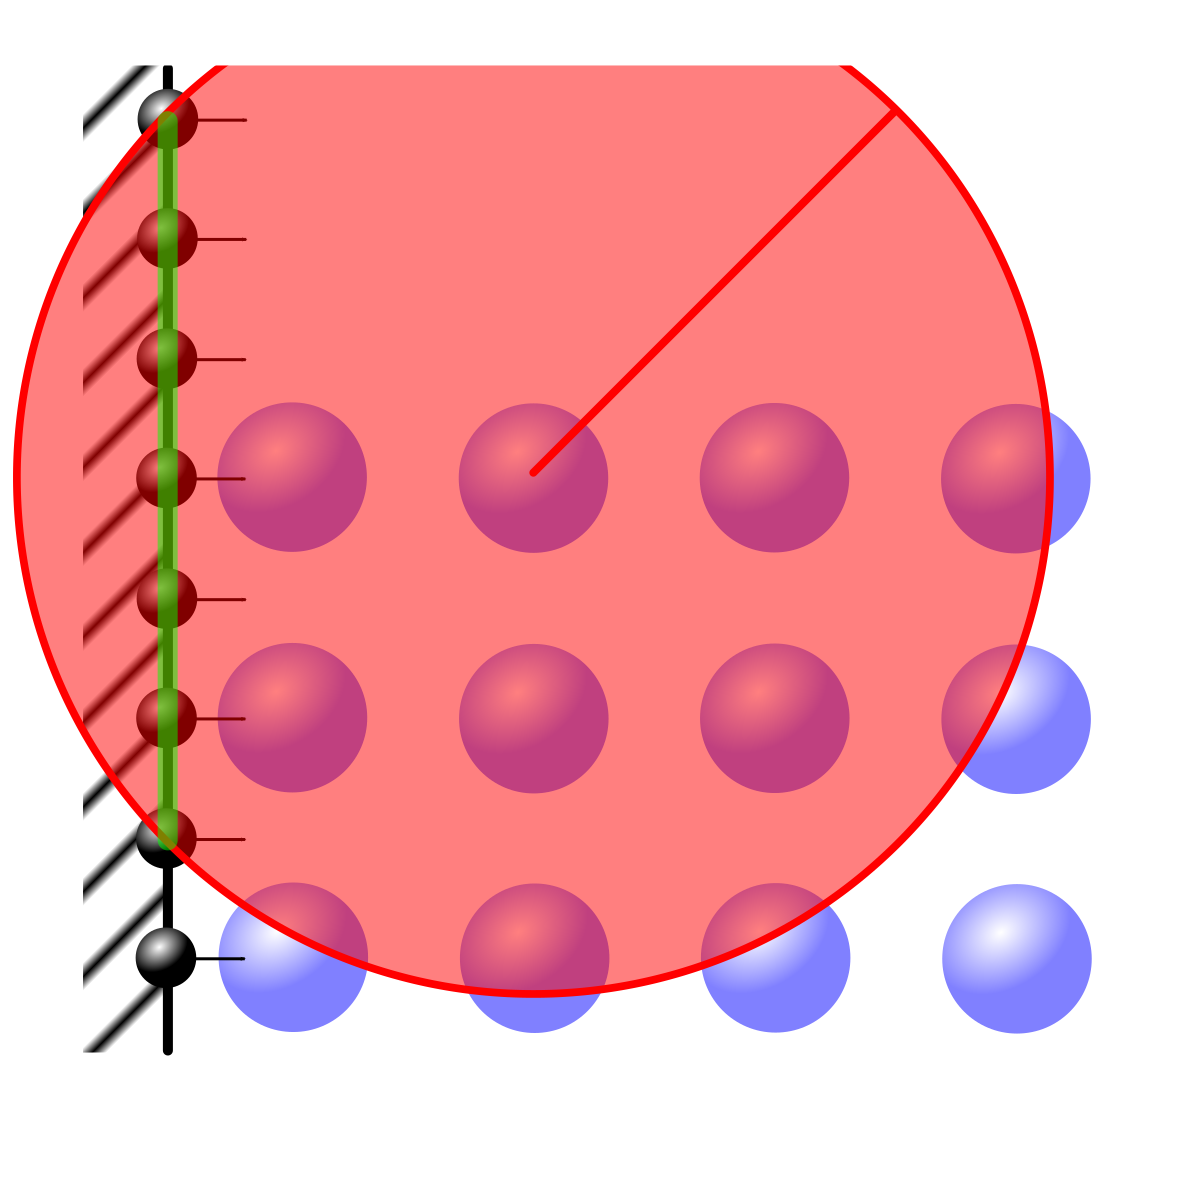
\includegraphics[width=0.4\textwidth]{DeLeffe}
  \caption{Boundary integrals scheme}
  \label{fig:aquagpusph:DeLeffeScheme}
\end{figure}
%
\begin{figure}[h!]
  \centering
  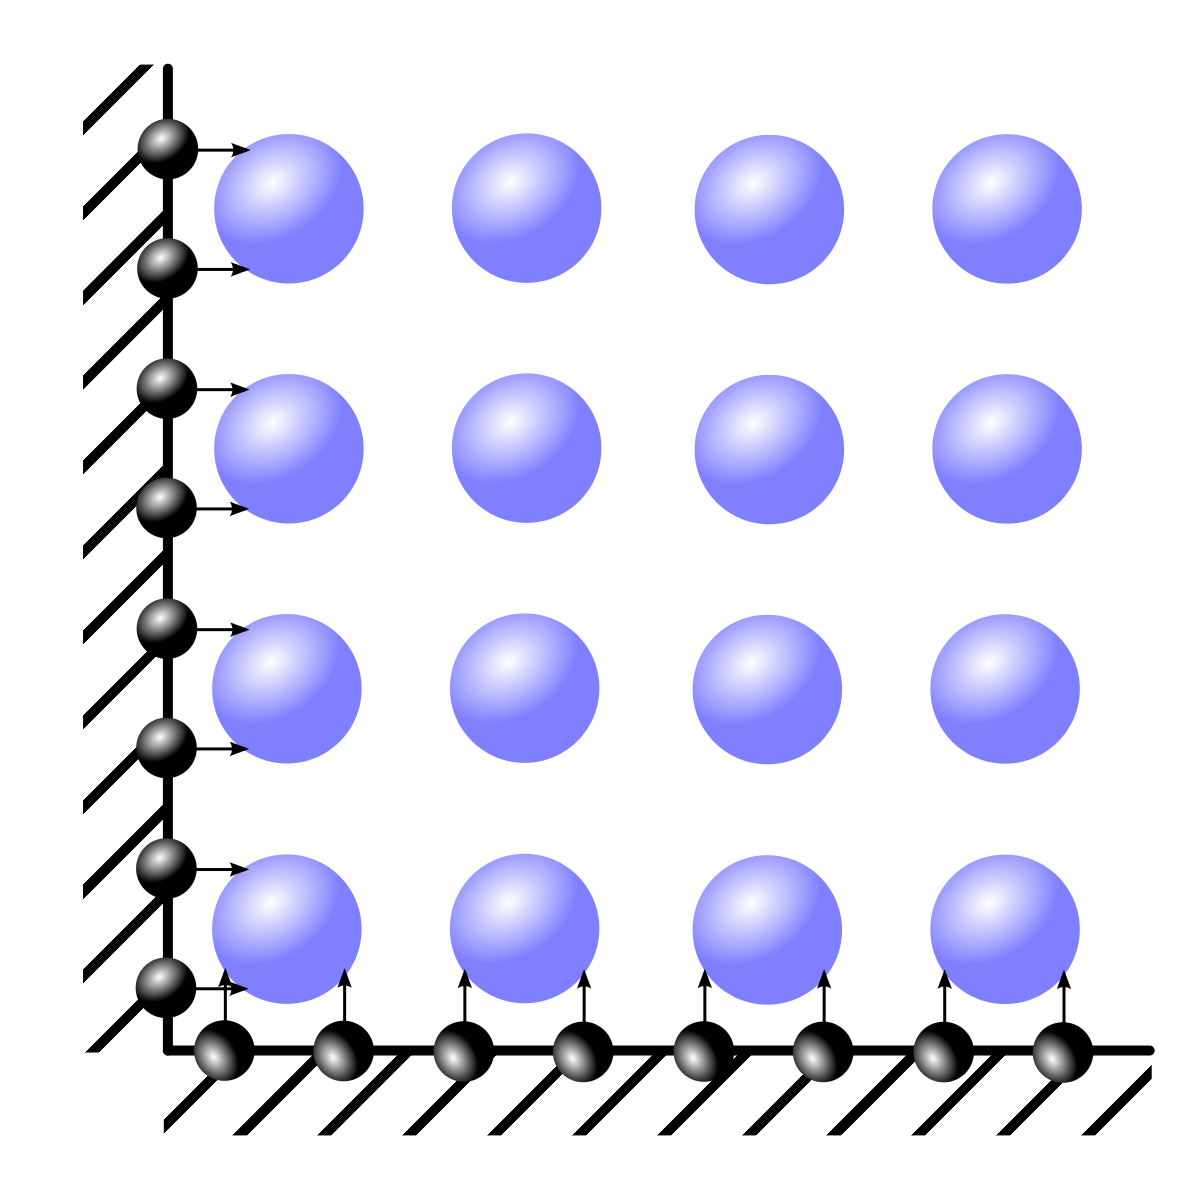
\includegraphics[width=0.4\textwidth]{DeLeffeCorner}
  \caption{Corner particles and vertexes distribution}
  \label{fig:aquagpusph:DeLeffeCorner}
\end{figure}
%
\subsection{Ghost particles}
\label{sss:aquagpusph:boundaries:ghostparticles}
%
`Ghost particles' is an algorithm so quite similar to `Fix particles' one, but in this case the extension of fluid
is not composed by particles linked to wall, that integrates their density using continuity equation, but is composed
by a mirroring of the fluid respect to the wall.\\
%
In the figure \ref{fig:aquagpusph:GhostParticlesScheme} a scheme about the fluid particles mirroring is shown.\\
%
So the SPH equation are therefore
%
\[
\left. \left\langle \frac{\gradient p}{\rho} \right\rangle_a \right\vert_{a \in \mathrm{Fluid}} = \frac{1}{\gamma_a}
	\sum\limits_{b \in \mathrm{Fluid}\;\cup\;\mathrm{Boundary}} 
		\left( \frac{p_a}{\rho_a^2} + \frac{p_b}{\rho_b^2} \right)
	\gradient W_{ab} m_b
\]
\[
\left. \left\langle \rho \; \divergence(v) \right\rangle_a \right\vert_{a \in \mathrm{Fluid}} =
	- \frac{1}{\gamma_a}
	\sum\limits_{b \in \mathrm{Fluid}\;\cup\;\mathrm{Boundary}} 
		\left( v_a - v_b \right)
	\gradient W_{ab} m_b
\]
\[
p_{a \in \mathrm{Boundary}} = \mathrm{f}\left(x_a, x_\mathrm{walls} \left( t \right) \right)
\]
\[
v_{a \in \mathrm{Boundary}} = \mathrm{f}\left(x_a, x_\mathrm{walls} \left( t \right) \right)
\]
%
The usual method to implement this boundary condition is perform a mirroring stage before the particles interaction,
storing the mirrored particles data in order to can use them within the fluid particles integration. In GPU
oriented code\footnote{and more generally for any parallel oriented one} this approach has the problem of the
previously unknown number of ghost particles, so memory reallocation or over-dimensioned arrays are mandatory
therefore. This can be walked around creating fix particles, but getting their values from fluid by a mirroring
operation and interpolation, with the advantage that the number of particles is ever know and reallocation is not
needed therefore, but with the disadvantage that requires to generate the fixed particles.\\
%
In \NAME a new algorithm is drafted, where the ghost particles are not precomputed, called `Virtual ghost particles'.
With this method a particles interaction process is called for each wall defined, so this method is not recommended
to high number of walls, nevertheless, when the particles interaction is called respect to a wall, each particle will
first test that is enough near to the wall before start working, so each `Ghost particles' interaction called is
significantly cheaper than usual one. The working method is locate all neighbours of the particle as is done on the
usual particles interaction method, and for each neighbour located compute the mirrored particle on runtime, avoiding
the need to store this data.\\
%
Since the number of walls must be relatively small, define the walls using particles with $imove < 0$ flag is not a
good option, so \NAME provides a parallel interface as has been described on chapter \ref{sss:XML:GhostParticles}.
This feature allows you to mix `Ghost particles' boundary condition with all other previous described, but probably
you only wants to mix it with `ElasticBounce boundary', in order to ensure than the fluid particles will not trespass
the walls.\\
%
`Ghost particles' boundary has the advantages of be easily defined in simple cases, and has been widely employed
along the SPH method history, so results can be easily compared. `Ghost particles' have some consistency problems
and is a condition bad defined in corners. When walls are perpendiculars the problem can be walked around adding
diagonal walls as shown in figure \ref{fig:aquagpusph:GhostParticlesCorner}, but for the moment general angles
intersection can not be solved in \NAME with `Ghost particles' boundary method yet.
%
\begin{figure}[h!]
  \centering
  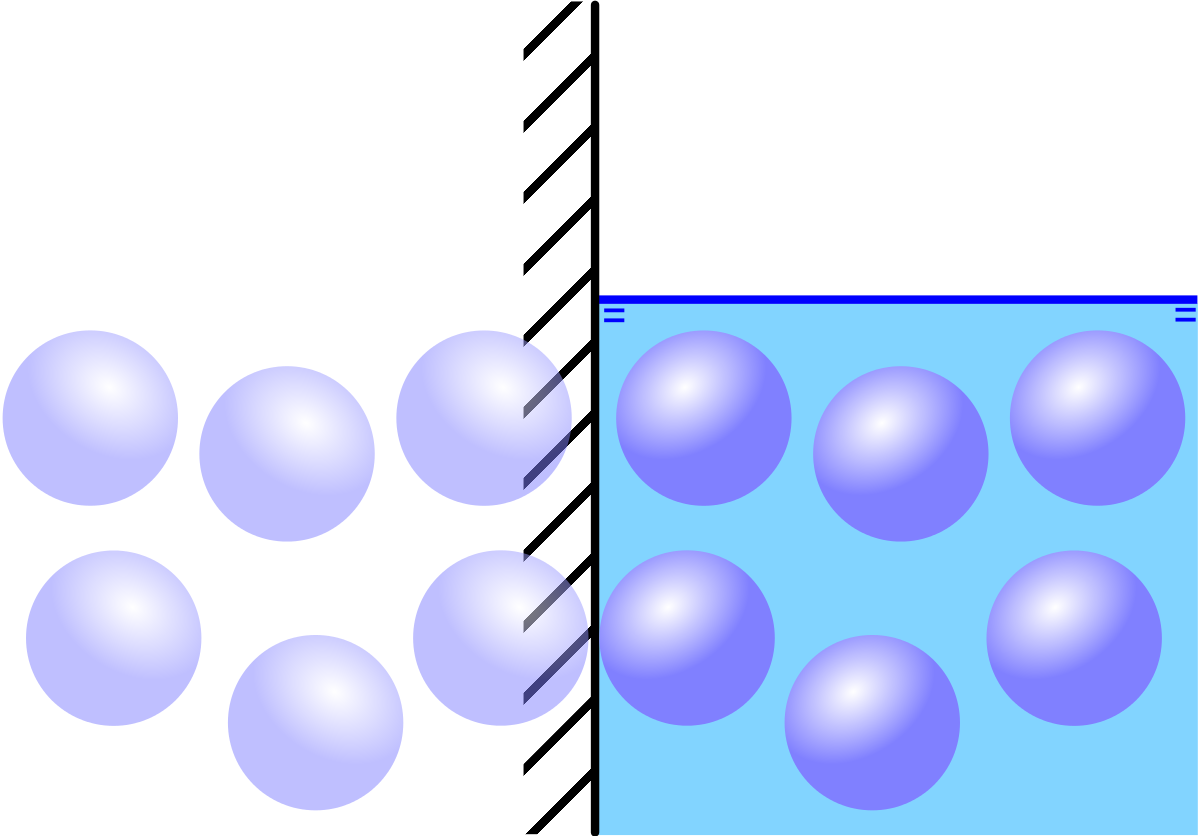
\includegraphics[width=0.4\textwidth]{GhostParticles}
  \caption{Ghost particles scheme}
  \label{fig:aquagpusph:GhostParticlesScheme}
\end{figure}
%
\begin{figure}[ht!]
  \centering
  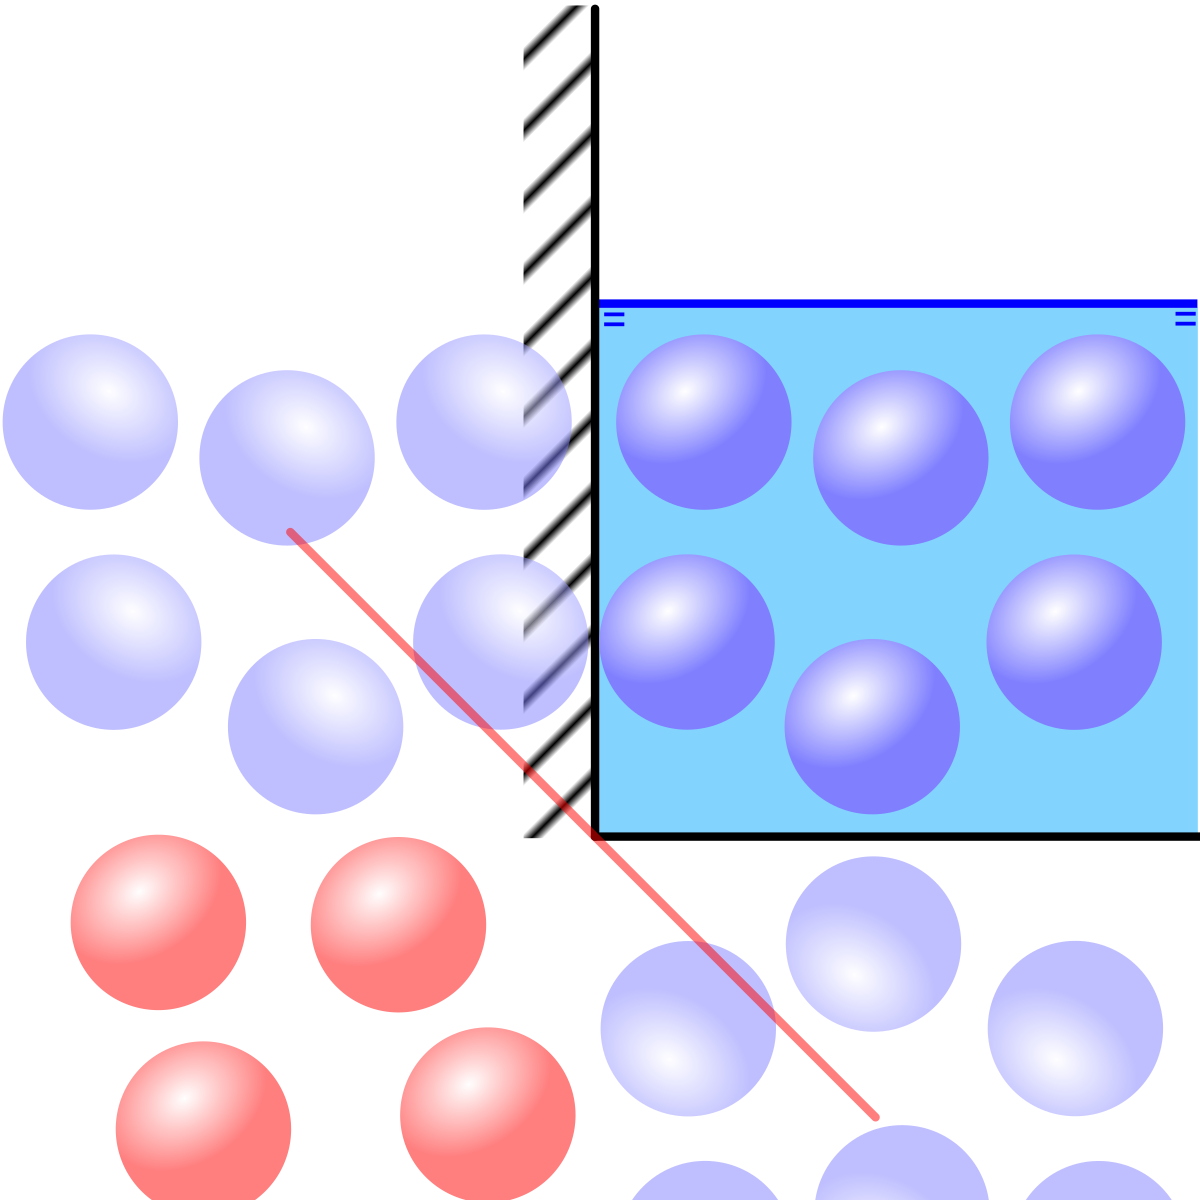
\includegraphics[width=0.4\textwidth]{GhostParticlesCorner}
  \caption{Ghost particles corner distribution}
  \label{fig:aquagpusph:GhostParticlesCorner}
\end{figure}
%

%
\section{Motions}
\label{ss:aquagpusph:motions}
%
\subsection{General}
%
In \NAME the motions imposed externally can be classified in 2 ways, by the method to impose the motion, and
by the method to compute the motion data. In table \ref{tables:aquagpusph:motions} all the available motions
in \NAME are listed, with their classification.\rc
%
Along this section all the different motion types, and control methods will be described. You can go to the
chapter \ref{s:examples} to see practical applications of some number of available motions.
%
\begin{table}[h!b!p!]\small
	\centering
	\begin{tabular}{| c | c | c | l | }
		\hline
		\cellcolor[rgb]{0.7,0.7,0.7}Movement & \cellcolor[rgb]{0.7,0.7,0.7}Motion type & \cellcolor[rgb]{0.7,0.7,0.7}Computation method \\
		\hline
		LIQuaternion     & Quaternion defined by axes & Linear interpolated data table \\
		\hline
		ScriptQuaternion & Quaternion defined by axes & Python script \\
		\hline
	\end{tabular}
	\caption{\NAME available motions.}
	\label{tables:aquagpusph:motions}
\end{table}
%
\subsection{Motion types}
\label{sss:aquagpusph:motions:Types}
%
\begin{center}
\textbf{Quaternion based motions}
\end{center}
%
The main method to impose motions in \NAME is to use Quaternions, that have the key feature that the motion is
ever fully described, not depending on any criteria. The problem with Quaternion imposed motions is that will
overwrite all the previous motions, so if you want to superpose several motions, Quaternion one must be the first.\\
%
When Quaternion motion is imposed in reality you are setting a movable reference coordinates, where object is fixed,
So in order to define instantaneous quaternion you must provide enough data to can describe it.
%
\begin{enumerate}
	\item 2D Simulations (AQUAgpusph2D)
	\begin{enumerate}
		\item \textbf{C.x}: x coordinate of the quaternion center.
		\item \textbf{C.y}: y coordinate of the quaternion center.
		\item \textbf{X.x}: x component of the X quaternion axis.
		\item \textbf{X.y}: y component of the X quaternion axis.
	\end{enumerate}
	\item 3D Simulations (AQUAgpusph)
	\begin{enumerate}
		\item \textbf{C.x}: x coordinate of the quaternion center.
		\item \textbf{C.y}: y coordinate of the quaternion center.
		\item \textbf{C.z}: z coordinate of the quaternion center.
		\item \textbf{X.x}: x component of the X quaternion axis.
		\item \textbf{X.y}: y component of the X quaternion axis.
		\item \textbf{X.z}: z component of the X quaternion axis.
		\item \textbf{Y.x}: x component of the Y quaternion axis.
		\item \textbf{Y.y}: y component of the Y quaternion axis.
		\item \textbf{Y.z}: z component of the Y quaternion axis.
	\end{enumerate}
\end{enumerate}
%
The undefined axis will be computed considering an orthonormal base. Provided axes will not be normalized, so
please ensure to provide right axes data.\\
%
Quaternion motions provided in \NAME will apply the motion over the particles with $imove \le 0$ flag (Fixed
particles or vertexes) and over defined walls as described on section \ref{sss:XML:GhostParticles}. You can
customize affected motion particles editing the provided Quaternion OpenCL kernel, but not walls for `Ghost
particles' boundary condition, that requires editing the \NAME source code.\\
%
In almost SPH simulations the time step is really small, for this reason in \NAME the velocity of the boundary
points (fixed particles, vertexes, or wall points) is determined as an euler derivation
%
\[v_{t+dt} = \frac{x_{t+dt} - x_t}{dt}\]
%
\subsection{Computation methods}
\label{sss:aquagpusph:motions:Controls}
%
\begin{center}
\textbf{Linear interpolated data table}
\end{center}
%
The simplest method to set the motion data is providing a tabulated file with the required data (see section
\ref{sss:aquagpusph:motions:Types} to know what data is required by the selected motion). Tabulated file
must contain one line per time instant with time at first column, and all the request fields by motion at the next
ones.\\
%
Comments can be included in the file with the symbol '\#'. All the line content after '\#' symbol will be
ignored. Fields can be separated by comma, semicolon, parenthesis, spaces or tabulator symbols, and if several
separators are concatenated between the field values then will be joined as a unique space separator.\\
%
When values are requested for a time instant $t$, such that $t_n < t < t_{n+1}$, values will be linearly interpolated
%
\[x(t) = \frac{t - t_n}{t_{n+1}-t_n} x(t_{n+1}) + \left( 1 - \frac{t - t_n}{t_{n+1}-t_n} \right) x(t_n)\]
%
You can see the section \ref{s:examples} to see practical application of linear interpolated tabulated motions data.
%
\begin{center}
\textbf{Python script controlled motion}
\end{center}
%
The most flexible and powerful method to control the motion is using a Python script where 2 methods must be
implemented:\\
%
\underline{\textbf{init}}\\
%
Method used to give the needed fields, as described on section \ref{sss:aquagpusph:motions:Types} for each type of
motion, for the time instant $t = 0 \mathrm{s}$, that can be useful to set initial condition.\\
%
\underline{\textbf{perform}}\\
%
Method called each time step in order to get all needed fields, as described on section
\ref{sss:aquagpusph:motions:Types} for each type of motion.
%
Input and output arguments may vary for both methods depending on the type of motion selected. We really encourage
user to go to chapter \ref{s:examples}, where practical applications of Python controlled motions can be found.
%
%
\section{Sensors}
\label{ss:aquagpusph:sensors}
%
In \NAME sensors are points where pressure and density fields will be measured. The method to add sensors into
the simulations has been described in the section \ref{sss:XML:Sensors}.\rc
%
Internally, the sensors are set as particles similar to the fluid ones, but with $imove = 0$ flag (fluid particles
have $imove > 0$ flag, and solid boundary elements $imove < 0$), and a null mass. The fields are interpolated in
the way described in section \ref{ss:sph_description}, where the discretized operators can be defined such that
%
\begin{eqnarray}
\label{eq:sensors:interpolation}
\langle p \rangle_a & = & \frac{1}{\gamma_a} \sum\limits_{b \in \mathrm{Fluid}} \frac{p_b}{\rho_b} W_{ab} m_b
\vspace{0.3cm} \\
\langle \rho \rangle_a & = & \frac{1}{\gamma_a} \sum\limits_{b \in \mathrm{Fluid}} W_{ab} m_b
\end{eqnarray}
%
Sensors measured values are ever renormalized with the Shepard correction ($\gamma_a$ is not forced to be equal to
1), even though Shepard correction has switched off for the forces and density rate computation, but in order to
you can revert the correction $\gamma_a$ (formerly $sumW$) is included into the output sensors data file.\rc
%
The sensors output data file is printed in the execution folder (so enough permissions are expected) with the name
``\textbf{Sensors.dat}'', inside the file a header will be printed, where the fields included are documented, and
then several rows (one per output time instant) with the following data distributed in columns:
%
\begin{enumerate}
	\item Time instant $t \mbox{[s]}$.
	\item Sensor data columns (one per sensor).
	\begin{enumerate}
		\item X position  $X \mbox{[m]}$.
		\item Y position  $Y \mbox{[m]}$.
		\item Z position  $Z \mbox{[m]}$ (only for 3D cases).
		\item Pressure $p \mbox{[Pa]}$.
		\item Density $\rho \mbox{[kg/m}^3\mbox{]}$.
		\item Kernel completeness factor $\gamma$.
	\end{enumerate}
\end{enumerate}
%
The fields are separated by tabulators. This file can be directly plot with gnuplot, or loaded easily with almost
data sheets.
%
%
